\documentclass{standalone}
\usepackage{tikz}
\usetikzlibrary{shapes.geometric, arrows.meta, positioning}

\begin{document}

% \begin{frame}{MPI Task Distribution for Full-Wave Simulation}

\centering
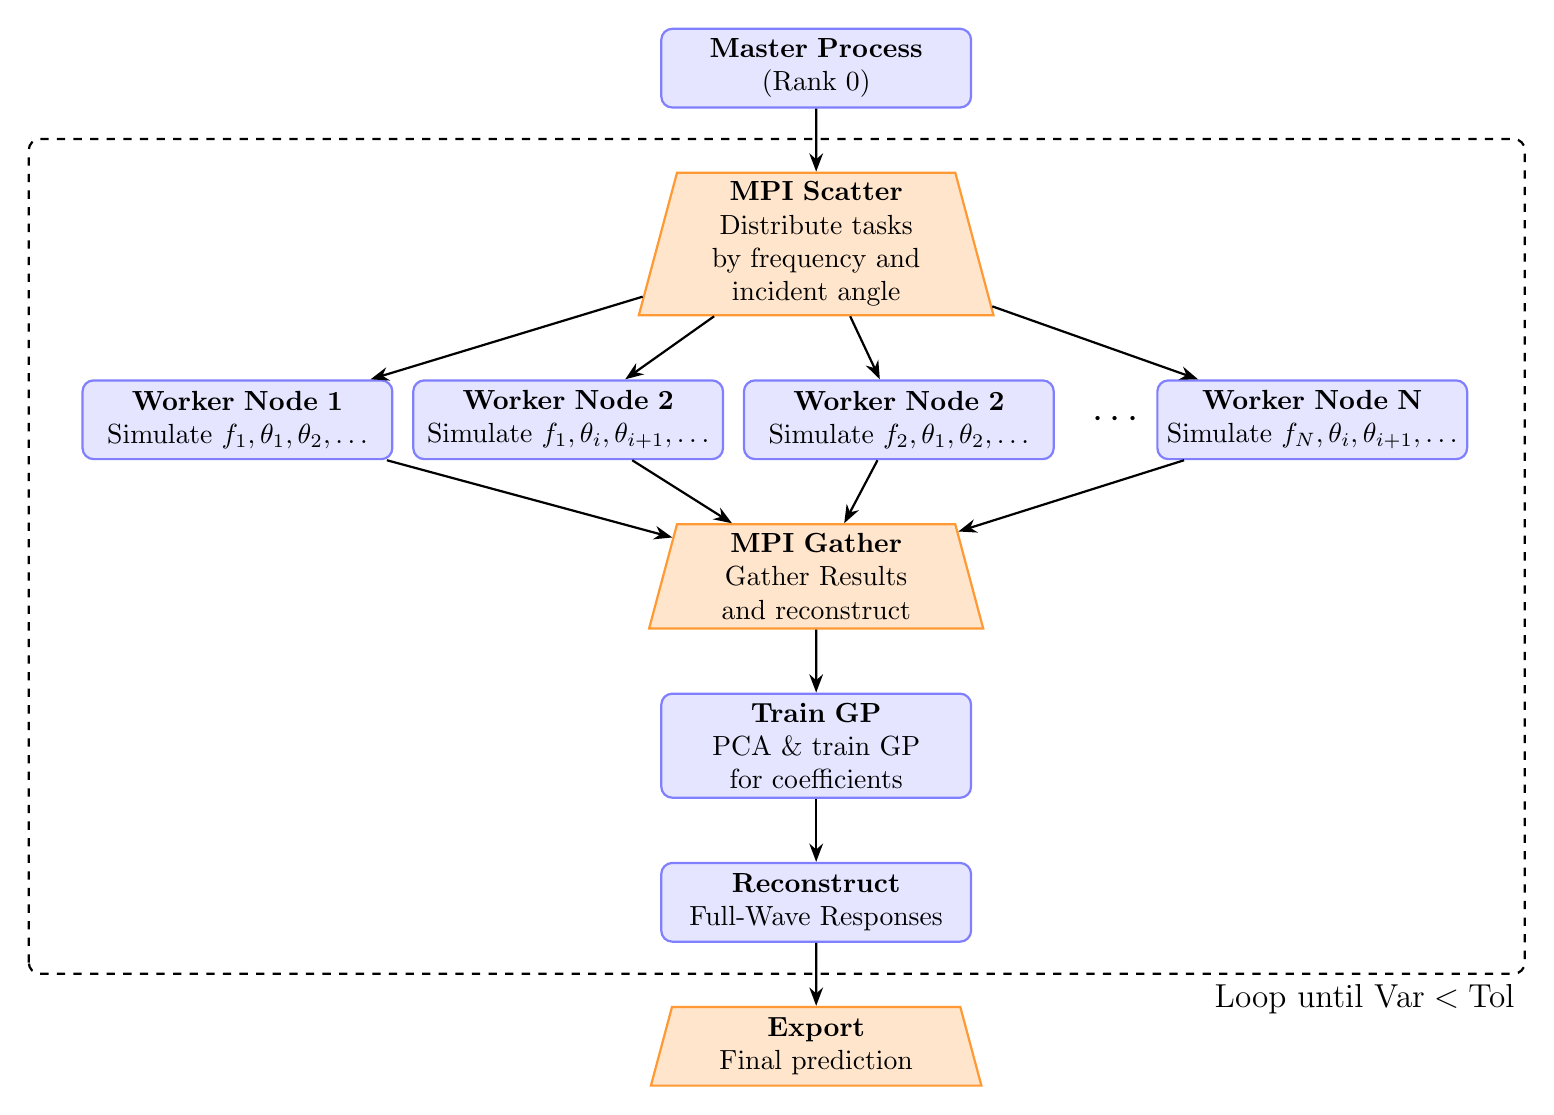
\begin{tikzpicture}[
  node distance=0.8cm and 1.0cm,
  process/.style={rectangle, rounded corners, draw=blue!50, fill=blue!10, thick, text width=3.7cm, align=center, minimum height=1cm},
  io/.style={trapezium, trapezium angle=75, draw=orange!80, fill=orange!20, thick, text width=3.3cm, align=center, minimum height=1cm},
  decision/.style={diamond, draw=green!50!black, fill=green!10, thick, text width=5cm, align=center, aspect=3},
  arrow/.style={-Stealth, thick}
]

\def\w{2.1cm};

% Nodes
\node[process] (master) {\textbf{Master Process} \\ (Rank 0)};

\node[io, below=of master] (distribute) {\textbf{MPI Scatter} \\ Distribute tasks \\ by frequency and \\ incident angle};
\node[process, below=of distribute, xshift={-3.5*\w}] (worker1) {\textbf{Worker Node 1} \\ Simulate $f_1, \theta_1, \theta_2, \dots$};
\node[process, below=of distribute, xshift={-1.5*\w}] (worker2) {\textbf{Worker Node 2} \\ Simulate $f_1, \theta_i, \theta_{i+1}, \dots$};
\node[process, below=of distribute, xshift={0.5*\w}] (worker3) {\textbf{Worker Node 2} \\ Simulate $f_2, \theta_1, \theta_2, \dots$};
\node[right=3.5mm of worker3] {\Large$\mathbf{\cdots}$};
\node[process, below=of distribute, xshift={3*\w}] (workerN) {\textbf{Worker Node N} \\ Simulate $f_N, \theta_i, \theta_{i+1}, \dots$};

\node[io, below=of worker2, xshift={1.5*\w}] (collect) {\textbf{MPI Gather} \\ Gather Results and reconstruct};
\node[process, below=of collect] (gp) {\textbf{Train GP} \\ PCA \& train GP for coefficients};
\node[process, below=of gp] (output) {\textbf{Reconstruct} \\ Full-Wave Responses};
\node[io, below=of output] (export) {\textbf{Export} \\ Final prediction};
% \node[decision, below=of output] (termination) {Variance $<$ tolerance ?};
% \node[io, below=of termination] (export) {\textbf{Export} \\ Final prediction};

% Arrows
\draw[arrow] (master) -- (distribute);
\draw[arrow] (distribute) -- (worker1);
\draw[arrow] (distribute) -- (worker2);
\draw[arrow] (distribute) -- (worker3);
\draw[arrow] (distribute) -- (workerN);
\draw[arrow] (worker1) -- (collect);
\draw[arrow] (worker2) -- (collect);
\draw[arrow] (worker3) -- (collect);
\draw[arrow] (workerN) -- (collect);
\draw[arrow] (collect) -- (gp);
\draw[arrow] (gp) -- (output);
\draw[arrow] (output) -- (export);
% \draw[arrow] (output) -- (termination);
% \draw[arrow] (termination) -- ++(10cm,0) -- ++(0,11cm) -- (distribute);
% \node[font=\small, right= 3mm of termination, yshift=-3mm] {no};
% \draw[arrow] (termination) -- (export) node[midway, right, font=\small] {yes};

\draw[black, thick, dashed, rounded corners=4pt] (-10cm, -11.5cm) rectangle (9cm, -0.9cm) node[pos=0.0, xshift=19cm, below left, font=\large] {Loop until $\mathrm{Var} < \mathrm{Tol}$};

% % Labels
% \node[draw, black, rounded corners=2pt, fill=white, above=0.3cm of distribute, text width=4cm, align=center, font=\small\bfseries] {MPI Scatter Phase};
% \node[draw, black, rounded corners=2pt, fill=white, below=0.25cm of collect, text width=4cm, align=center, font=\small\bfseries] {MPI Gather Phase};

\end{tikzpicture}

% \end{frame}

\end{document}
